\begin{name}
	{\tenchude}
	{TOÁN 11}
	{LỚP TOÁN THẦY PHÁT}
	{Thời gian: 90 phút - Không kể thời gian phát đề}
\end{name}
\setcounter{ex}{0}\setcounter{bt}{0}
\noindent{\bf\fontfamily{qag}\selectfont\color{violet}A. PHẦN TRẮC NGHIỆM}
\Opensolutionfile{ans}[ans/ans-1-GK1-KNTT-14-NH23-24]
\begin{ex}%[0H3B6-2]% ::Cau 1::
	Với góc $\alpha $ bất kì, đẳng thức nào sau đây là đúng?
	\choice
	{$\cos \left( \pi-\alpha \right)=\cos \alpha $}
	{\True $\cos \left( \pi-\alpha \right)=-\cos \alpha $}
	{$\sin \left( \pi-\alpha \right)=-\sin \alpha $}
	{$\tan \left( \pi-\alpha \right)=\tan \alpha $}
	\loigiai{
		Ta có $\cos \left( \pi-\alpha \right)=-\cos \alpha $, $\sin \left( \pi-\alpha \right)=\sin \alpha $, $\tan \left( \pi-\alpha \right)=-\tan \alpha $.\\
		Do đó ta chọn phương án $\cos \left( \pi-\alpha \right)=-\cos \alpha $.}
\end{ex}
\begin{ex}%[0H3B5-2]% ::Cau 2::
	Biết góc $\alpha $ thỏa mãn $\cos \alpha =\dfrac{2}{3}$. Hỏi $\alpha $ có thể nhận giá trị trong khoảng nào dưới đây?
	\choice
	{$\left( \dfrac{\pi}{2};\dfrac{2\pi}{3} \right)$}
	{$\left( \dfrac{8\pi}{3};\dfrac{17\pi}{6} \right)$}
	{\True $\left( \dfrac{\pi}{4};\dfrac{\pi}{3} \right)$}
	{$\left( -\pi;-\dfrac{2\pi}{3} \right)$}
	\loigiai{
		Vì $\cos \alpha =\dfrac{2}{3}$ nên $\alpha \in \left( -\dfrac{\pi}{2}+k2\pi,\dfrac{\pi}{2}+k2\pi \right)$ với $k\in \mathbb{Z}$.\\
		Với $k=0$ thì $\alpha\in \left(-\dfrac{\pi}{2};\dfrac{\pi}{2}\right)$. Vì $\left( \dfrac{\pi}{4};\dfrac{\pi}{3} \right)\subset \left(-\dfrac{\pi}{2};\dfrac{\pi}{2}\right)$.\\
		Do đó, ta chọn phương án $\left( \dfrac{\pi}{4};\dfrac{\pi}{3} \right)$.}
\end{ex}
\begin{ex}%[0H3Y5-2]% ::Cau 3::
	Cho góc $\alpha $ thỏa $-\dfrac{3\pi}{2}<\alpha <-\pi$. Tìm mệnh đề đúng trong các mệnh đề sau:
	\choice
	{$\cos \alpha >0$}
	{$\cot \alpha >0$}
	{\True $\sin \alpha >0$}
	{$\tan \alpha >0$}
	\loigiai{
		\begin{center}
			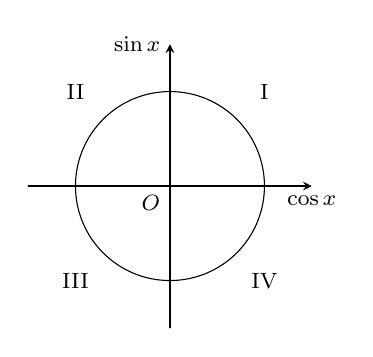
\begin{tikzpicture}[scale=1.2,font=\footnotesize,line join=round,line cap=round,>=stealth]
				\path 	
				(0,0) coordinate (O)
				(1,0) coordinate (A)
				(-1,0) coordinate (A')
				(0,1) coordinate (B)
				(0,-1) coordinate (B')
				;		
				\draw[-stealth] (-1.5,0)--(1.5,0)node[below]{$\cos x$};
				\draw[-stealth] (0,-1.5)--(0,1.5)node[left]{$\sin x$};
				\draw (O) node[below left]{$O$}  circle (1);
				\draw (1,1) node{I} (-1,1) node{II} (-1,-1) node{III} (1,-1)node{IV} ;
%				\foreach \x/\g in {A/30,B/45,A'/120,B'/-30}
%				\fill[black] 	(\x) circle (1pt)
%				($(\g:3mm)+(\x)$) node {$\x$};
			\end{tikzpicture}
		\end{center}
		Do $-\dfrac{3\pi}{2}<\alpha <-\pi$ nên điểm $M$ biểu diễn góc lượng giác có số đo $\alpha $ thuộc góc phần tư số II. \\
		Do đó $\sin \alpha >0$, $\cos \alpha <0$, $\tan \alpha <0$, $\cot \alpha <0$.}
\end{ex}
\begin{ex}%[0H3B5-2]% ::Cau 4::
	Cho $\cot \alpha =4\tan \alpha $ và $\alpha \in \left( \dfrac{\pi}{2};\pi \right)$. Khi đó $\sin \alpha $ bằng
	\choice
	{$-\dfrac{\sqrt{5}}{5}$}
	{$\dfrac{1}{2}$}
	{$\dfrac{2\sqrt{5}}{5}$}
	{\True $\dfrac{\sqrt{5}}{5}$}
	\loigiai{
		Ta có 
		\allowdisplaybreaks
		\begin{eqnarray*}
		&& \cot \alpha =4\tan \alpha \\
		&\Leftrightarrow& \dfrac{\cot \alpha }{\tan \alpha }=4\\
		&\Leftrightarrow& \cot^2 \alpha =4\Leftrightarrow 1+\cot^2 \alpha =5\\
		&\Leftrightarrow& \dfrac{1}{{\sin ^2}\alpha }=5\\
		&\Leftrightarrow& {\sin ^2}\alpha =\dfrac{1}{5}\\
		&\Leftrightarrow& \sin \alpha =\pm \dfrac{\sqrt{5}}{5}.
		\end{eqnarray*}
		Vì $\alpha \in \left( \dfrac{\pi}{2};\pi \right)$ nên $\sin \alpha =\dfrac{\sqrt{5}}{5}$.}
\end{ex}
\begin{ex}%[0H3Y6-2]% ::Cau 5::
	Khẳng định nào sau đây là \textbf{sai}?
	\choice
	{$\cos 2a=2\cos^2 a-1$}
	{$\cos 2a=\cos^2 a-{\sin ^2}a$}
	{$\sin 2a=2\sin a\cos a$}
	{\True $\cos 2a=2{\sin ^2}a-1$}
	\loigiai{
		Theo công thức nhân đôi ta có $\cos 2a=1-2{\sin ^2}a$.}
\end{ex}
\begin{ex}%[0H3Y6-2]% ::Cau 6::
	Khẳng định nào sau đây là \textbf{sai}?
	\choice
	{$\cos a+\cos b=2\cos \dfrac{a+b}{2}\cos \dfrac{a-b}{2}$}
	{\True $\cos a-\cos b=2\sin \dfrac{a+b}{2}\sin \dfrac{a-b}{2}$}
	{$\sin a+\sin b=2\sin \dfrac{a+b}{2}\cos \dfrac{a-b}{2}$}
	{$\sin a-\sin b=2\cos \dfrac{a+b}{2}\sin \dfrac{a-b}{2}$}
	\loigiai{
		Theo công thức biến tổng thành tích ta có $\cos a-\cos b=-2\sin \dfrac{a+b}{2}\cdot\sin \dfrac{a-b}{2}$.}
\end{ex}
\begin{ex}%[0H3B5-2]% ::Cau 7::
	Cho $\tan \alpha +\cot \alpha =m$. Tính giá trị của biểu thức $\tan^3 \alpha +\cot^3 \alpha $
	\choice
	{$m^3+3m$}
	{$3m^3+m$}
	{$3m^3-m$}
	{\True $m^3-3m$}
	\loigiai{
		Ta có
		\allowdisplaybreaks
		\begin{eqnarray*}
		\tan^3 \alpha +\cot^3 \alpha &=& \left( \tan \alpha +\cot \alpha \right)\left( \tan^2 \alpha -\tan \alpha \cdot\cot \alpha +\cot^2 \alpha \right)\\
		&=& \left( \tan \alpha +\cot \alpha \right)\left[ \left( \tan \alpha +\cot \alpha \right)^2-3\tan \alpha \cdot\cot \alpha \right]\\
		&=& \left( \tan \alpha +\cot \alpha \right)\cdot\left[ \left( \tan \alpha +\cot \alpha \right)^2-3 \right]\\
		&=& m\left( m^2-3 \right)=m^3-3m.
		\end{eqnarray*}
	}
\end{ex}
\begin{ex}%[1D1Y1-1]% ::Cau 8::
	Tìm tập xác định $\mathscr{D}$ của hàm số $y=\dfrac{2023}{\sin x}$.
	\choice
	{$\mathscr{D}=\mathbb{R}\setminus \left\{\dfrac{\pi}{2}+k\pi\,\middle|\, k\in \mathbb{Z} \right\}$}
	{$\mathscr{D}=\mathbb{R}\setminus \left\{\dfrac{k\pi}{2} \,\middle|\, k\in \mathbb{Z} \right\}$}
	{$\mathscr{D}=\mathbb{R}\setminus \left\{0 \right\}$}
	{\True $D=\mathbb{R}\setminus \left\{k\pi\,\middle|\, k\in \mathbb{Z} \right\}$}
	\loigiai{
		Điều kiện xác định $\sin x\ne 0\Leftrightarrow x\ne k\pi,k\in \mathbb{Z}$.\\
	Vậy $\mathscr{D}=\mathbb{R}\setminus \left\{k\pi\,\middle|\, k\in \mathbb{Z}  \right\}$.}
\end{ex}
\begin{ex}%[1D1Y1-3]% ::Cau 9::
	Cho hàm số $y=\tan x$. Khẳng định sau đây là \textbf{sai}?
	\choice
	{\True Hàm số đã cho là hàm số chẵn}
	{Tập xác định của hàm số đã cho là $\mathbb{R}\setminus \left\{\dfrac{\pi}{2}+k\pi\,\middle|\, k\in \mathbb{Z} \right\}$}
	{Hàm số đã cho đồng biến trên mỗi khoảng $\left( -\dfrac{\pi}{2}+k\pi;\dfrac{\pi}{2}+k\pi \right)$ với $k\in \mathbb{Z}$}
	{Hàm số đã cho tuần hoàn theo chu kì $\pi$}
	\loigiai{
	Hàm số $y=\tan x$ là hàm số lẻ.
	}
\end{ex}
\begin{ex}%[1D1Y1-6]% ::Cau 10::
	Trong các hàm số sau, hàm số nào có đồ thị như hình vẽ bên dưới?
	\begin{center}
		\begin{tikzpicture}[scale=1,font=\footnotesize,line join=round,line cap=round,>=stealth]		
			\draw[-stealth] (-6.7,0)--(6.7,0)node[below]{$x$};
			\draw[-stealth] (0,-1.2)--(0,2)node[left]{$y$};
			\draw (0,0) node[below right]{$O$};
			\draw[thick,smooth,samples=200] plot[domain=-6.6:6.6] (\x,{sin (\x*180/pi)});
			\draw[fill=black]  (-6.28,0) circle (1pt) node [above left] {$-2\pi$};
			\draw[fill=black]  (-4.71,0) circle (1pt) node [below] {$-\dfrac{3\pi}{2}$};
			\draw[fill=black]  (-3.14,0) circle (1pt) node [above] {$-\pi$};
			\draw[fill=black] (-1.57,0) circle (1pt) node [above] {$-\dfrac{\pi}{2}$};
			\draw[fill=black]  (1.57,0) circle (1pt) node [below] {$\dfrac{\pi}{2}$};
			\draw[fill=black]  (3.14,0) circle (1pt) node [above] {$\pi$};
			\draw[fill=black]  (4.71,0) circle (1pt) node [above] {$\dfrac{3\pi}{2}$};
			\draw[fill=black]  (6.28,0) circle (1pt) node [above] {$2\pi$};
			\draw (0,1) node[above right] {$1$} (0,-1) node[below right] {$-1$};
			\draw[dashed] (-6.7,-1)--(6.7,-1) (-6.7,1)--(6.7,1);
			\draw[dashed] (-1.57,0)--(-1.57,-1) (1.57,0)--(1.57,1) (4.71,0)--(4.71,-1) (-4.71,0)--(-4.71,1);
		\end{tikzpicture}
	\end{center}
	\choice
	{\True $y=\sin x$}
	{$y=\cos x$}
	{$y=\tan x$}
	{$y=\cot x$}
	\loigiai{
		Từ hình vẽ ta thấy hàm số có miền giá trị từ $-1$ đến $1$, tuần hoàn với chu kỳ $2\pi$ và nhận gốc tọa độ làm tâm đối xứng nên đây là đồ thị của hàm số $y=\sin x$.}
\end{ex}
\begin{ex}%[1D1B1-4]% ::Cau 11::
	Tìm chu kì $T$ của hàm số $y=2\cos^2 x+2023$.
	\choice
	{$T=3\pi$}
	{$T=2\pi$}
	{\True $T=\pi$}
	{$T=4\pi$}
	\loigiai{
		Ta có $y=2\cos^2 x+2023=\cos 2x+2024$.\\
		Vậy hàm số có chu kì $T=\pi$.}
\end{ex}
\begin{ex}%[1D1K1-1]% ::Cau 12::
	Tập xác định $\mathscr{D}$ của hàm số $y=\sqrt{4+\sin x}-\dfrac{1+x}{\tan^2 \left( x-\dfrac{\pi}{4} \right)-1}+3\tan \left( x+\dfrac{\pi}{4} \right)$ là
	\choice
	{$\mathscr{D}=\mathbb{R}\setminus \left\{\dfrac{\pi}{4}+k\dfrac{\pi}{2},k\in \mathbb{Z} \right\}$}
	{$\mathscr{D}=\mathbb{R}\setminus \left\{k\dfrac{\pi}{2},k\in \mathbb{Z} \right\}$}
	{\True $\mathscr{D}=\mathbb{R}\setminus \left\{k\dfrac{\pi}{4},k\in \mathbb{Z} \right\}$}
	{$\mathscr{D}=\mathbb{R}\setminus \left\{\dfrac{\pi}{4}+k\pi,k\in \mathbb{Z} \right\}$}
	\loigiai{
		Do $-1\le \sin x\le 1$ nên $4+\sin x>0$, $\,\forall x\in \mathbb{R}$.\\
		Hàm số xác định khi và chỉ khi\\
		$\heva{
			& x-\dfrac{\pi}{4}\ne \dfrac{\pi}{2}+m\pi\\
			& \tan^2 \left( x-\dfrac{\pi}{4} \right)\ne 1 \\
			& x+\dfrac{\pi}{4}\ne \dfrac{\pi}{2}+q\pi\\
		}\Leftrightarrow \heva{
			& x\ne \dfrac{3\pi}{4}+m\pi\\
			& x-\dfrac{\pi}{4}\ne \dfrac{\pi}{4}+n\pi\\
			& x-\dfrac{\pi}{4}\ne -\dfrac{\pi}{4}+p\pi\\
			& x\ne \dfrac{\pi}{4}+q\pi\\
		}\Leftrightarrow \heva{
			& x\ne \dfrac{3\pi}{4}+m\pi\\
			& x\ne \dfrac{\pi}{2}+n\pi\\
			& x\ne p\pi\\
			& x\ne \dfrac{\pi}{4}+q\pi\\
		}\Leftrightarrow x\ne k\dfrac{\pi}{4},\,\left( m,n,p,q,k\in \mathbb{Z} \right)$.\\
		Vậy tập xác định $\mathscr{D}=\mathbb{R}\setminus \left\{k\dfrac{\pi}{4},k\in \mathbb{Z} \right\}$.}
\end{ex}
\begin{ex}%[1D1B2-1]% ::Cau 13::
	Giải phương trình $\cos \left( x-\dfrac{\pi}{6} \right)=\dfrac{1}{2}$.
	\choice
	{$\hoac{
			& x=\dfrac{\pi}{3}+k2\pi\\
			& x=k2\pi\\
		}\,\left( k\in \mathbb{Z} \right)$}
	{$\hoac{
			& x=\dfrac{\pi}{2}+k\pi\\
			& x=-\dfrac{\pi}{6}+k\pi\\
		}\left( k\in \mathbb{Z} \right)$}
	{$\hoac{
			& x=\dfrac{\pi}{2}+k2\pi\\
			& x=\dfrac{\pi}{6}+k2\pi\\
		}\left( k\in \mathbb{Z} \right)$}
	{\True $\hoac{
			& x=\dfrac{\pi}{2}+k2\pi\\
			& x=-\dfrac{\pi}{6}+k2\pi\\
		}\left( k\in \mathbb{Z} \right)$}
	\loigiai{
		Ta có $\cos \left( x-\dfrac{\pi}{6} \right)=\dfrac{1}{2}\Leftrightarrow \hoac{
			& x-\dfrac{\pi}{6}=\dfrac{\pi}{3}+k2\pi\\
			& x-\dfrac{\pi}{6}=-\dfrac{\pi}{3}+k2\pi\\
		}\Leftrightarrow \hoac{
			& x=\dfrac{\pi}{2}+k2\pi\\
			& x=-\dfrac{\pi}{6}+k2\pi\\
		}\left( k\in \mathbb{Z} \right)$.}
\end{ex}
\begin{ex}%[1D1B2-1]% ::Cau 14::
	Phương trình $\sin 2x=-\dfrac{1}{2}$ có tập nghiệm là
	\choice
	{$\hoac{
			& x=\dfrac{7\pi}{12}+k\pi\\
			& x=-\dfrac{7\pi}{12}+k\pi\\
		}\left( k\in \mathbb{Z} \right)$}
	{$\hoac{
			& x=\dfrac{\pi}{12}+k2\pi\\
			& x=-\dfrac{7\pi}{12}+k2\pi\\
		}\left( k\in \mathbb{Z} \right)$}
	{$\hoac{
			& x=\dfrac{\pi}{12}+k\pi\\
			& x=\dfrac{7\pi}{12}+k\pi\\
		}\left( k\in \mathbb{Z} \right)$}
	{\True $\hoac{
			& x=-\dfrac{\pi}{12}+k\pi\\
			& x=\dfrac{7\pi}{12}+k\pi\\
		}\left( k\in \mathbb{Z} \right)$}
	\loigiai{
		Ta có $\sin 2x=-\dfrac{1}{2}\Leftrightarrow \hoac{
			& 2x=-\dfrac{\pi}{6}+k2\pi\\
			& 2x=\dfrac{7\pi}{6}+k2\pi\\
		}\Leftrightarrow \hoac{
			& x=-\dfrac{\pi}{12}+k\pi\\
			& x=\dfrac{7\pi}{12}+k\pi\\
		}\left( k\in \mathbb{Z} \right)$.}
\end{ex}
\begin{ex}%[1D1B2-1]% ::Cau 15::
	Phương trình $\sin \left( 2x-\dfrac{\pi}{4} \right)=\sin \left( x+\dfrac{3\pi}{4} \right)$ có tổng các nghiệm thuộc khoảng $\left( 0;\pi \right)$ bằng
	\choice
	{$\dfrac{7\pi}{2}$}
	{\True $\pi$}
	{$\dfrac{3\pi}{2}$}
	{$\dfrac{\pi}{4}$}
	\loigiai{
		Ta có $$\sin \left( 2x-\dfrac{\pi}{4} \right)=\sin \left( x+\dfrac{3\pi}{4} \right)\Leftrightarrow \hoac{
			& 2x-\dfrac{\pi}{4}=x+\dfrac{3\pi}{4}+k2\pi\\
			& 2x-\dfrac{\pi}{4}=\dfrac{\pi}{4}-x+l2\pi}
		\Leftrightarrow \hoac{
			& x=\pi+k2\pi\\
			& x=\dfrac{\pi}{6}+l\dfrac{2\pi}{3}},\left( k,l\in \mathbb{Z} \right).$$
		Họ nghiệm $x=\pi+k2\pi$ không có nghiệm nào thuộc khoảng $\left( 0;\pi \right)$.\\
		Với $x=\dfrac{\pi}{6}+l\dfrac{2\pi}{3}\in \left( 0;\pi \right)\Rightarrow 0<\dfrac{\pi}{6}+l\dfrac{2\pi}{3}<\pi\Leftrightarrow l\in \left\{0;1 \right\}$.\\
		Vậy phương trình có hai nghiệm thuộc khoảng $\left( 0;\pi \right)$ là $x=\dfrac{\pi}{6}$ và $x=\dfrac{5\pi}{6}$. \\
		Từ đó suy ra tổng các nghiệm thuộc khoảng $\left( 0;\pi \right)$ của phương trình này bằng $\pi$.}
\end{ex}
\begin{ex}
	Khai triển $\cos 4 \alpha$ theo $\cos \alpha$ ta được biểu thức $a\cos^4 \alpha +b\cos^2 \alpha +c$. Giá trị biểu thức $a-b+c$ bằng
	\choice
	{$13$}
	{\True $17$}
	{$-11$}
	{$-15$}
	\loigiai{
Ta có $\cos 4 \alpha =2\cos^2 2\alpha -1= 2 \left(2\cos^2 \alpha -1\right)^2 -1 = 8\cos^4 \alpha -8\cos^2 \alpha +1$.
}
\end{ex}
\begin{ex}%[1K1K4-3]%Câu 27
    Cho hai phương trình $\cos 3x-1=0$; $\cos 2x=-\dfrac{1}{2}$. Các giá trị nào dưới đây là nghiệm chung của hai phương trình đã cho?
    \choice
        {$x=\dfrac{\pi }{3}+k2\pi, k\in \mathbb{Z}$}
        {$x=k2\pi, k\in \mathbb{Z}$}
        {$x=\pm \dfrac{\pi }{3}+k2\pi, k\in \mathbb{Z}$}
        {\True $x=\pm \dfrac{2\pi }{3}+k2\pi, k\in \mathbb{Z}$}
    \loigiai{
        Ta có 
        \begin{itemize}
            \item $\cos 3x-1=0\Leftrightarrow \cos 3x=1
            \Leftrightarrow x=k\dfrac{2\pi }{3}, k\in \mathbb{Z}$.
            \item $\cos 2x=-\dfrac{1}{2}
            \Leftrightarrow 2x=\pm \dfrac{2\pi }{3}+k2\pi \Leftrightarrow x=\pm \dfrac{\pi }{3}+k\pi,k\in \mathbb{Z}.$
        \end{itemize}
        Biểu diễn các nghiệm trên đường tròn lượng giác ta có tập các nghiệm của hai phương trình là $x=\pm \dfrac{2\pi }{3}+k\pi, k\in \mathbb{Z}$.}
\end{ex}
\begin{ex}%[1K1B2-3]%Câu 21
    Biểu thức $\dfrac{\sin 10^\circ +\sin 20^\circ}{\cos 10^\circ +\cos 20^\circ}$ bằng $a\tan b$ với $a,b\in \mathbb{N}$ và $b\in [0;180]$. Tính $a+b$. 
    \choice
        {$88$}
        {$69$}
        {$29$}
        {\True $16$}
    \loigiai{
        $\dfrac{\sin 10^\circ+\sin 20^\circ}{\cos 10^\circ+\cos 20^\circ}=\dfrac{2\sin 15^\circ\cos 5^\circ}{2\cos 15^\circ\cos 5^\circ}=\tan 15^\circ$.}
\end{ex}
\begin{ex}%[1D3Y4-3]% ::Cau 16::
	Cho cấp số nhân $(u_n)$ có số hạng đầu $u_1=4$ và công bội $q=2$. Số hạng thứ $10$ của cấp số nhân đó là
	\choice
	{$u_{10}=2^{12}$}
	{\True $u_{10}=2^{11}$}
	{$u_{10}=2^{10}$}
	{$u_{10}=2^9$}
	\loigiai{
	Ta có $u_{10}=u_1\cdot q^{10-1}=4\cdot 2^9=2^2\cdot 2^9=2^{11}$.
	}
\end{ex}
\begin{ex}%[1D3B4-2]% ::Cau 17::
	Cho cấp số nhân $(u_n)$ với $u_1=-3;u_6=96$. Công bội của cấp số nhân đó là
	\choice
	{\True $q=-2$}
	{$q=-3$}
	{$q=2$}
	{$q=3$}
	\loigiai{
	Ta có $u_6=u_1q^5 \Rightarrow q^5=\dfrac{u_6}{u_1}=\dfrac{96}{-3}=-32$, suy ra $q=-2$.}
\end{ex}
\begin{ex}%::Cau 18::
	Công ty muốn ước lượng tỉ lệ các cỡ áo khi may cho học sinh lớp 11 đã đo chiều cao của 36 học sinh nam khối 11 của một trường và thu được mẫu số liệu sau (đơn vị là centimét):
	\begin{center}
		\begin{tabular}{lllllllllllll}
			160 & 161 & 161 & 162 & 162 & 162 & 163 & 163 & 163 & 164 & 164 & 164 & 164 \\ 
			165 & 165 & 165 & 165 & 165 & 166 & 166 & 166 & 166 & 167 & 167 & 168 & 168 \\ 
			168 & 168 & 169 & 169 & 170 & 171 & 171 & 172 & 172 & 174 & & & 
		\end{tabular}
	\end{center}
	Biết rằng học sinh có chiều cao thuộc $[160;167)$ sẽ mua cỡ áo M. Có bao nhiêu học sinh mua cỡ áo M?
	\choice
	{\True $22$}
	{$6$}
	{$15$}
	{$20$}
	\loigiai{
	Bảng tần số ghép nhóm
			\begin{center}
				\begin{tabular}{|c|c|c|c|c|c|}
					\hline Chiều cao $(\mathrm{cm})$ & {$[150 ; 160)$} & {$[160 ; 167)$} & {$[167 ; 170)$} & {$[170 ; 175)$} & {$[175 ; 180)$} \\
					\hline Số học sinh &0& 22 & 8 & 6 & 0 \\
					\hline
				\end{tabular}
			\end{center}
	}
\end{ex}
\begin{ex}%:Cau 19::
	Tìm tứ phân vị thứ nhất và thứ ba (làm tròn đến hàng phần chục) của mẫu số liệu sau 
	\begin{center}
		\begin{tabular}{|c|c|c|c|c|c|}
			\hline Chiều cao $(\mathrm{cm})$ & {$[150 ; 160)$} & {$[160 ; 167)$} & {$[167 ; 170)$} & {$[170 ; 175)$} & {$[175 ; 180)$} \\
			\hline Số học sinh &5& 17 & 8 & 6 & 0 \\
			\hline
		\end{tabular}
	\end{center}
	\choice
	{$Q_1 \approx 159{,}2$, $Q_3 \approx 169{,}8$}
	{\True $Q_1 \approx 161{,}6$, $Q_3 \approx 168{,}9$}
	{$Q_1 \approx 160{,}2$, $Q_3 \approx 170{,}3$}
	{$Q_1 \approx 163{,}6$, $Q_3 \approx 171{,}4$}
	\loigiai{
	\begin{itemize}
		\item $\dfrac{n}{4}=9$, $p=2$, $a_2=160$, $m_1=5$, $m_2=17$, $a_3-a_2=7$. $$Q_1=160 + \dfrac{9-5}{17} \cdot 7 \approx 161{,}6.$$
		\item $\dfrac{3n}{4}=27$, $p=3$, $a_3=167$, $m_1+m_2=22$, $m_3=8$, $a_4-a_3=3$. $$Q_3=167 + \dfrac{27-22}{8} \cdot 3 \approx 168{,}9$$
	\end{itemize}
	}
\end{ex}
\begin{ex}%[1D3Y2-2]% ::Cau 20::
	Cho dãy số $(u_n)$ với $u_n=\dfrac{n+1}{n-2}$. Tính $u_{20}$.
	\choice
	{\True $\dfrac{21}{18}$}
	{$\dfrac{18}{21}$}
	{$\dfrac{11}{8}$}
	{$\dfrac{8}{11}$}
	\loigiai{
		Ta có $u_{20}=\dfrac{20+1}{20-2}=\dfrac{21}{18}$.}
\end{ex}
\begin{ex}%[1D3B4-2]% ::Cau 21::
	Cho cấp số nhân có $u_1=2$ và $u_6=486$. Tìm công bội của cấp số nhân.
	\choice
	{$1$}
	{\True $3$}
	{$2$}
	{$4$}
	\loigiai{
		Ta có $u_6=u_1\cdot q^5\Rightarrow {q^5}=\dfrac{u_6}{u_1}=\dfrac{486}{2}=243=3^5\Rightarrow q=3$.}
\end{ex}
\begin{ex}%[0D5BC-1]% ::Cau 22::
	Cho mẫu số liệu ghép nhóm về thống kê chiều cao (mét) của $35$ cây bạch đàn trong rừng, ta có bảng số liệu sau:
	\begin{center}
		\begin{tabular}{|c|c|c|c|c|}
			\hline
		Khoảng chiều cao (m)	& $[6{,5};7)$ & $[7;7{,5})$ & $[7{,}5;8)$ & $[8;8{,}5)$ \\
			\hline
		Số cây	& $6$ & $15$ & $11$ & $3$ \\
			\hline
		\end{tabular}
	\end{center}
	Tính chiều cao trung bình của $35$ cây bạch đàn trên. (Kết quả làm tròn đến hàng phần nghìn).
	\choice
	{\True $7{,}407$ m}
	{$4{,}707$ m}
	{$7{,}704$ m}
	{$7{,}5$ m}
	\loigiai{
		Ta có giá trị đại diện các nhóm được cho dưới bảng sau:
		\begin{center}
			\begin{tabular}{|c|c|c|c|c|}
				\hline
				Khoảng chiều cao (m)	& $[6{,5};7)$ & $[7;7{,5})$ & $[7{,}5;8)$ & $[8;8{,}5)$ \\
				\hline
				Giá trị đại diện	& $6{,}75$	&$7{,}25$&$7{,}75$	&$8{,}25$	\\
				\hline
				Tần số (Số cây)	& $6$ & $15$ & $11$ & $3$ \\
				\hline
			\end{tabular}
		\end{center}
		Từ đó suy ra chiều cao trung bình của 35 cây bạch đàn là
		$$\overline{x}=\dfrac{6{,}75\cdot 6+7{,}25\cdot 15+7{,}75\cdot 11+8{,}25\cdot 3}{35}=7{,}047 \,\text{m}.$$}
\end{ex}
\begin{ex}%[0D5BC-3]% ::Cau 23::
	Tìm hiểu thời gian hoàn thành một bài tập (đơn vị: phút) của một số học sinh thu được kết quả sau:
	\begin{center}
		\begin{tabular}{|c|c|c|c|c|c|}
			\hline
		Thời gian (phút)	& $[0;4)$ & $[4;8)$ & $[8;12)$ & $[12;16)$ & $[16;20)$ \\
			\hline
		Số học sinh	& $2$ & $4$ & $7$ & $4$ & $3$ \\
			\hline
		\end{tabular}
	\end{center}
	Tứ phân vị thứ ba của mẫu số liệu ghép nhóm này là
	\choice
	{$Q_3=13$}
	{\True $Q_3=14$}
	{$Q_3=15$}
	{$Q_3=12$}
	\loigiai{
		Cỡ mẫu: $n=2+4+7+4+3=20$.\\
		Tứ phân vị thứ ba $Q_3$ là $\dfrac{x_{15}+x_{16}}{2}$. \\
		Do ${x_{15}},{x_{16}}$ đều thuộc nhóm $\left[ 12;16 \right)$ nên nhóm này chứa $Q_3$.\\
		Do đó $p=4$, $a_4=12$, $m_4=4$, $m_1+m_2+m_3=2+4+7=13$, $a_5-a_4=4$. \\
		Ta có $Q_3=12+\dfrac{\dfrac{3\cdot 20}{4}-13}{4}\cdot 4=14$.}
\end{ex}
\begin{ex}%[0D5YC-1]% ::Cau 24::
	Một nhóm 10 học sinh có điểm thi môn toán là: $5$; $6$; $7$; $5$; $8$; $8$; $10$; $9$; $7$; $8$. Tính điểm trung bình của nhóm học sinh trên.
	\choice
	{$8$}
	{\True $7{,}3$}
	{$8{,}3$}
	{$7{,}7$}
	\loigiai{
		Điểm trung bình là $\overline{x}=\dfrac{5\cdot 2+6+7\cdot 2+8\cdot 3+9+10}{10}=7{,}3$.}
\end{ex}
\begin{ex}%[0D5YC-2]% ::Cau 25::
	Thời gian xem ti vi trong tuần (đơn vị: giờ) của một số học sinh thu được kết quả như sau:
	\begin{center}
	\begin{tabular}{|c|c|c|c|c|c|}
		\hline
		Thời gian (giờ)	& $[0;4)$ & $[4;8)$ & $[8;12)$ & $[12;16)$ & $[16;20)$ \\
		\hline
		Số học sinh	& $6$ & $12$ & $4$ & $4$ & $2$ \\
		\hline
	\end{tabular}
	\end{center}
	Giá trị đại diện của nhóm $\left[ 12;16 \right)$ là
	\choice
	{$12$}
	{\True $14$}
	{$10$}
	{$16$}
	\loigiai{
	Giá trị đại diện của nhóm $\left[ 12;16 \right)$ là $\dfrac{12+16}{2}=14$.
	}
\end{ex}
\begin{ex}%[1D3Y2-2]% ::Cau 26::
	Cho dãy số $u_n$ biết với $u_n=\dfrac{1}{n+1}$, ba số hạng đầu tiên của dãy đó là
	\choice
	{\True $\dfrac{1}{2};\dfrac{1}{3};\dfrac{1}{4}$}
	{$1;\dfrac{1}{2};\dfrac{1}{3}$}
	{$\dfrac{1}{2};\dfrac{1}{4};\dfrac{1}{6}$}
	{$1;\dfrac{1}{3};\dfrac{1}{5}$}
	\loigiai{
	Ta có $u_n=\dfrac{1}{n+1}$, khi đó $u_1=\dfrac{1}{1+1}=\dfrac{1}{2}$, $u_2=\dfrac{1}{2+1}=\dfrac{1}{3}$, $u_3=\dfrac{1}{3+1}=\dfrac{1}{4}$.\\
	Ba số hạng đầu tiên của dãy đó là $\dfrac{1}{2};\dfrac{1}{3};\dfrac{1}{4}$.
	}
\end{ex}
\begin{ex}%[1D3B3-6]% ::Cau 27::
	Người ta trồng $465$ cây trong một khu vườn hình tam giác như sau: Hàng thứ nhất có $1$ cây, hàng thứ hai có $2$ cây, hàng thứ ba có $3$ cây. Số hàng cây trong khu vườn là:
	\choice
	{$31$}
	{\True $30$}
	{$29$}
	{$28$}
	\loigiai{
		Cách trồng $465$ cây trong một khu vườn hình tam giác như trên lập thành một cấp số cộng $\left( {u_n} \right)$ với số $u_n$ là số cây ở hàng thứ $n$ và $u_1=1$ và công sai $d=1$.\\
		Tổng số cây trồng được là
		$$S_n=465\Leftrightarrow \dfrac{n\left( n+1 \right)}{2}=465\Leftrightarrow {n^2}+n-930=0\Leftrightarrow \hoac{
			& n=30 \\
			& n=-31\,\left( \text{loại} \right).}$$
		Như vậy số hàng cây trong khu vườn là $30$.}
\end{ex}
\begin{ex}%[1D3B3-5]% ::Cau 28::
	Cho cấp số cộng $\left( u_n \right)$ có $u_{27}+u_2=83$. Khi đó tổng $28$ số hạng đầu tiên của cấp số cộng $\left( u_n \right)$ là
	\choice
	{\True $S_{28}=1162$}
	{$S_{28}=1612$}
	{$S_{28}=2611$}
	{$S_{28}=1261$}
	\loigiai{
		Gọi $d$ và $u_1$ lần lượt là công sai và số hạng đầu của cấp số cộng $\left( {u_n} \right)$\\
		Ta có $S_{28}=\dfrac{28\left( u_1+u_{28} \right)}{2}=\dfrac{28\left( u_2-d+u_{27}+d \right)}{2}=\dfrac{28\left( u_2+u_{27} \right)}{2}=\dfrac{28\cdot 83}{2}=1162$.}
\end{ex}
\begin{ex}%[1D3B3-2]% ::Cau 29::
	Cho cấp số cộng $\left( u_n \right)$ biết $u_{27}=-76$ và $u_{83}=-244$. Khi đó số hạng đầu $u_1$ của cấp số cộng đã cho bằng
	\choice
	{$-3$}
	{$5$}
	{$4$}
	{\True $2$}
	\loigiai{
		Gọi $d$ là công sai của cấp số cộng đã cho.\\
		Áp dụng công thức $u_n=u_1+\left( n-1 \right)d$, ta có 
		$$\heva{
			& u_{27}=-76 \\
			& u_{83}=-244}
		\Leftrightarrow \heva{
			& u_1+26d=-76 \\
			& u_1+82d=-244}
		\Leftrightarrow \heva{
			& u_1=2 \\
			& d=-3.}$$}
\end{ex}
\begin{ex}%[1D3K3-4]% ::Cau 30::
	Cho $a<b<c$ là ba số nguyên. Biết $a$, $b$, $c$ theo thứ tự tạo thành một cấp số cộng và $a$, $c$, $b$ theo thứ tự tạo thành một cấp số nhân. Tìm giá trị nhỏ nhất của $c$.
	\choice
	{$-2$}
	{\True $2$}
	{$-1$}
	{$4$}
	\loigiai{
		Ta có $\heva{& 2b=a+c \\& c^2=ab>0}$. Suy ra $$2c^2=a\left( a+c \right)\Rightarrow 2c^2-ac-a^2=0\Rightarrow \hoac{
			& c=a\,\left( \text{loại} \right) \\
			& c=-\dfrac{a}{2}\Rightarrow b=\dfrac{a}{4}=-\dfrac{c}{2}.}$$
		Suy ra $a$, $b$ trái dấu với $c$ $\Rightarrow \heva{
			& a<0 \\
			& c>0.}$\\
		Do $a$, $b$, $c$ nguyên nên $c$ chia hết cho $2$.\\
		Do đó $c$ nhỏ nhất bằng $2$ khi đó $a=-4$, $b=-1$.}
\end{ex}
\begin{ex}%[Dự án 1 - TLDH - TeamTeXHoa - Lê Quân]%[1K2B5-1] 
	Cho dãy số $(u_n)$ có $u_n=2\cdot 3^n$. Công thức truy hồi của dãy số $(u_n)$ là 
	\choice
	{$\heva{&u_1=6	\\&u_n=6u_{n-1},\, \forall n>1}$}
	{\True $\heva{&u_1=6	\\&u_n=3u_{n-1},\, \forall n>1}$}
	{$\heva{&u_1=3	\\&u_n=3u_{n-1},\, \forall n>1}$}
	{$\heva{&u_1=3	\\&u_n=6u_{n-1},\, \forall n>1}$}
	\loigiai{
		Ta có $u_n=2\cdot 3^n\Rightarrow \heva{&u_1=2\cdot 3^1=6	\\&u_{n+1}=2\cdot 3^{n+1}.}$\\
		$\Rightarrow u_{n+1}=2\cdot3\cdot 3^n =3u_n\Rightarrow u_n=3\cdot u_{n-1}$.\\
		Vậy $\heva{&u_1=6	\\&u_n=3u_{n-1},\, \forall n>1.}$
	}
\end{ex}
\begin{ex}%[Dự án 1 - TLDH - TeamTeXHoa - Sauluoi3105]%[1K2B5-4]
	Cho dãy số $\left(u_n\right)$, với $u_n=\dfrac{1}{1\cdot 4}+\dfrac{1}{2\cdot 5}+\ldots+\dfrac{1}{n(n+3)}, \forall n=1 ; 2 ; 3 \cdots$. Mệnh đề nào sau đây đúng?
	\choice
	{Dãy số $\left(u_n\right)$ bị chặn trên và không bị chặn dưới}
	{Dãy số $\left(u_n\right)$ bị chặn dưới và không bị chặn trên}
	{\True Dãy số $\left(u_n\right)$ bị chặn}
	{Dãy số $\left(u_n\right)$ không bị chặn}
	\loigiai{
		Ta có $u_n>0$ suy ra $\left(u_n\right)$ bị chặn dưới bởi $0$.\\ 
		Mặt khác $\dfrac{1}{k(k+3)}<\dfrac{1}{k(k+1)}=\dfrac{1}{k}-\dfrac{1}{k+1}\left(k \in \mathbb{N}^*\right)$ nên 
		$$u_n<\dfrac{1}{1\cdot 2}+\dfrac{1}{2\cdot 3}+\dfrac{1}{3\cdot 4}+\cdots+\dfrac{1}{n(n+1)}=1-\dfrac{1}{2}+\dfrac{1}{2}-\dfrac{1}{3}+\dfrac{1}{2}-\dfrac{1}{4}+\cdots+\dfrac{1}{n}-\dfrac{1}{n+1}=1-\dfrac{1}{n+1}<1.$$
Suy ra dãy $\left(u_n\right)$ bị chặn trên.\\
Vậy dãy $\left(u_n\right)$ bị chặn.
	}
\end{ex}
\Closesolutionfile{ans}
% \inputans{10}{ans/ans-1-GK1-KNTT-14-NH23-24}
\noindent{\bf\fontfamily{qag}\selectfont\color{violet}B. PHẦN TỰ LUẬN}
\setcounter{bt}{0}
\begin{bt}%[1D1B2-1]% ::Cau 31::
	% \begin{enumEX}{1}
		% \item 
		Cho $\alpha \in (-\dfrac{\pi}{2};0)$ và $\sin \alpha = -\dfrac13$. Tìm $\cos \alpha$, $\tan \alpha$, $\cot \alpha$. 
		% \item Giải phương trình $\cot \left( 2x-40^{\circ} \right)=-\sqrt{3}$.
	% \end{enumEX}
	\loigiai{
		% \begin{enumEX}{1}
		% \item 
		Ta có $\alpha \in (-\dfrac{\pi}{2};0)$ nên $\cos \alpha >0$. Suy ra $$\cos^2 \alpha = 1-\sin^2 \alpha = 1-\left(-\dfrac13\right)=\dfrac89 \Rightarrow \cos \alpha = \dfrac{2\sqrt{2}}{3}.$$ 
		$\tan \alpha = \dfrac{\sin \alpha}{\cos \alpha} = \dfrac{-\dfrac13}{\dfrac{2\sqrt{2}}{3}}=-\dfrac{\sqrt{2}}{4}$.\\
		$\cot \alpha = \dfrac{1}{\tan \alpha} = -2\sqrt{2}$.
		% \item Ta có $\cot \left( 2x-40^{\circ} \right)=-\sqrt{3}\Leftrightarrow 2x-40^{\circ} =-30^{\circ} +k180^{\circ} \Leftrightarrow x=5^{\circ} +k90^{\circ} ,\,\left( k\in \mathbb{Z} \right)$.
	% \end{enumEX}
	}
\end{bt}

\begin{bt}%[1D3B3-3]% ::Cau 34::
	Tìm tổng $15$ số hạng đầu tiên của cấp số cộng $\left( {u_n} \right)$, biết $\heva{& u_1+u_5-u_3=10 \\& u_1+u_6=17.}$
	\loigiai{
	Ta có
		$$\heva{
			& {u_1}+u_5-u_3=10 \\
			& {u_1}+u_6=17}
		\Leftrightarrow \heva{
			& {u_1}+u_1+4d-\left( {u_1}+2d \right)=10 \\
			& {u_1}+u_1+5d=17}
		\Leftrightarrow \heva{
			& {u_1}+2d=10 \\
			& 2u_1+5d=17}
		\Leftrightarrow \heva{
			& u_1=16 \\
			& d=-3.}$$
		Suy ra $S_{15}=\dfrac{15}{2}\left(2u_1+14d\right)=\dfrac{15}{2}[2 \cdot 16 + 14\cdot (-3)]=-150$.}
\end{bt}

\begin{bt}%[1D1K3-8]% ::Cau 36::
	Hàng ngày mực nước của một con kênh lên xuống theo thủy triều. Độ sâu $h$ (mét) của mực nước trong kênh tính theo thời gian $t$ (giờ) $\left( 0\le t\le 24 \right)$ được mô tả bởi công thức $h=A\cos \left( \dfrac{\pi t}{6}+1 \right)+B$, với $A, B$ là các số thực dương cho trước. Biết độ sâu của mực nước lớn nhất là $15$ mét khi thủy triều lên cao và khi thủy triều xuống thấp thì độ sâu của mực nước thấp nhất là $9$ mét. Tính thời điểm độ sâu của mực nước là $13{,}5$ mét (tính chính xác đến $\dfrac{1}{100}$ giờ).
	\loigiai{
		Với mọi $0\le t\le 24$, ta có
		\allowdisplaybreaks
		\begin{eqnarray*}
		&& -1\le \cos \left( \dfrac{\pi t}{6}+1 \right)\le 1 \\
		&\Leftrightarrow& -A+B\le A\cos \left( \dfrac{\pi t}{6}+1 \right)+B\le A+B.
		\end{eqnarray*}
		Độ sâu của mực nước lớn nhất bằng $A+B$ khi $\cos \left( \dfrac{\pi t}{6}+1 \right)=1$ và thấp nhất bằng $-A+B$ khi $\cos \left( \dfrac{\pi t}{6}+1 \right)=-1$.\\
		Ta có hệ $\heva{
			& A+B=15 \\
			& -A+B=9}
		\Leftrightarrow \heva{
			& B=12 \\
			& A=3.}$\\
		Ta được $h=3\cos \left( \dfrac{\pi t}{6}+1 \right)+12$.\\
		Theo đề, ta tìm thời điểm mà độ sâu 
		\allowdisplaybreaks
		\begin{eqnarray*}
		&& h=13{,}5\Leftrightarrow 3\cos \left( \dfrac{\pi t}{6}+1 \right)+12=13{,}5\Leftrightarrow \cos \left( \dfrac{\pi t}{6}+1 \right)=\dfrac{1}{2}\\
		&\Leftrightarrow& \hoac{
			& \dfrac{\pi t}{6}+1=\dfrac{\pi}{3}+k2\pi\\
			& \dfrac{\pi t}{6}+1=-\dfrac{\pi}{3}+k2\pi},\left( k\in \mathbb{Z} \right)
		\Leftrightarrow \heva{
			& t=\left( -1+\dfrac{\pi}{3} \right)\cdot \dfrac{6}{\pi}+12k \\
			& t=\left( -1-\dfrac{\pi}{3} \right)\cdot \dfrac{6}{\pi}+12k},\left( k\in \mathbb{Z} \right).
		\end{eqnarray*}
		Do $0\le t\le 24; k\in \mathbb{Z}$ nên $t=0{,}09$ (giờ); $t=12{,}09$ (giờ); $t=8{,}09$ (giờ); $t=20{,}09$ (giờ).}
\end{bt}

	\begin{bt}%[Trần Ngọc Thành, CTST-BG11]%[1T3T1-6]
		Cho hình vuông $H_0$ cạnh bằng 1 đơn vị độ dài. Chia hình vuông $H_0$ thành chín hình vuông bằng nhau, bỏ đi bốn hình vuông, nhận được hình $H_1$. Tiếp theo, chia mỗi hình vuông của $H_1$ thành chín hình vuông, rồi bỏ đi bốn hình vuông, nhận được hình $H_2$. Tiếp tục quá trình này, ta nhận được một dãy hình $H_n$ $(n=1,2,3,\ldots)$.	
		\\
		\centerline{
			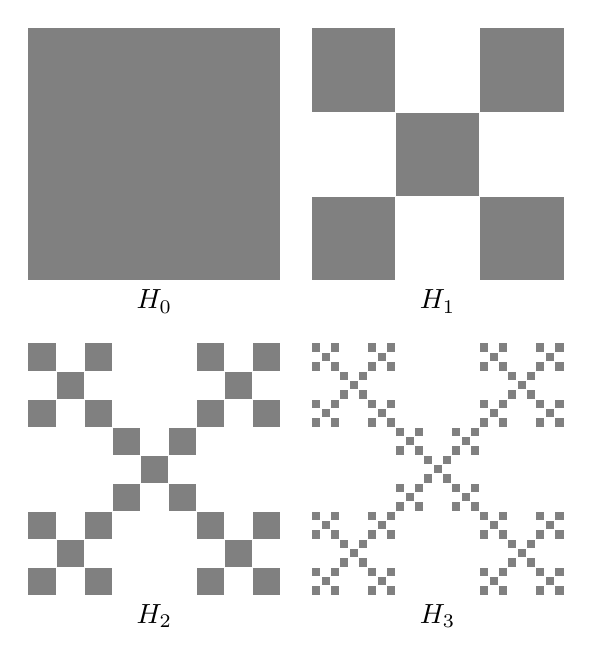
\begin{tikzpicture}[scale=.8]% Muốn vẽ hình Hn thì dùng \hv{n}
				\def\a{2}
				\pgfmathsetmacro\sh{2*\a *sqrt(2)/3}
				\def\hv#1{
					\ifnum#1>0
					\draw[white,fill=white] 
					(-\a/3,\a/3) rectangle (\a/3,\a)
					(-\a/3,-\a/3) rectangle (-\a,\a/3)
					(-\a/3,-\a/3) rectangle (\a/3,-\a)
					(\a/3,-\a/3) rectangle (\a,\a/3)
					;
					\pgfmathtruncatemacro{\k}{#1-1}
					\begin{scope}[scale=1/3]\hv{\k}\end{scope}
					\begin{scope}[shift={(45:\sh)},scale=1/3]\hv{\k}\end{scope}
					\begin{scope}[shift={(135:\sh)},scale=1/3]\hv{\k}\end{scope}
					\begin{scope}[shift={(225:\sh)},scale=1/3]\hv{\k}\end{scope}
					\begin{scope}[shift={(315:\sh)},scale=1/3]\hv{\k}\end{scope}
					\fi
				}
				\begin{scope}
					\fill[gray] (-\a,-\a) rectangle (\a,\a);
					\hv{0}
					\path (0,-\a)node[below]{$H_0$};
				\end{scope}
				\begin{scope}[xshift=4.5cm]
					\fill[gray] (-\a,-\a) rectangle (\a,\a);
					\hv{1}
					\path (0,-\a)node[below]{$H_1$};
				\end{scope}
				\begin{scope}[yshift=-5cm]
					\fill[gray] (-\a,-\a) rectangle (\a,\a);
					\hv{2}
					\path (0,-\a)node[below]{$H_2$};
				\end{scope}
				\begin{scope}[xshift=4.5cm,yshift=-5cm]
					\fill[gray] (-\a,-\a) rectangle (\a,\a);
					\hv{3}
					\path (0,-\a)node[below]{$H_3$};
				\end{scope}
				% \path (current bounding box.south) node[below]{Hình $6$};
			\end{tikzpicture}
		}
		Tính tổng diện tích và tổng chu vi tất cả hình vuông được tô màu trong hình $H_5$.
		\loigiai{
			\begin{enumerate}
				\item Hình vuông $H_1$ có diện tích $S_1=5\cdot \left(\dfrac{1}{3}\right)^2=\dfrac{5}{9}$.\\
				Hình vuông $H_2$ có diện tích $S_2=5^2\cdot \left(\dfrac{1}{3^2}\right)^2=\left(\dfrac{5}{9}\right)^2$.\\
				Hình vuông $H_n$ có diện tích $S_n=5^n\cdot \left(\dfrac{1}{3^n}\right)^2=\left(\dfrac{5}{9}\right)^n$.\\
				
				\item Hình vuông $H_1$ có chu vi $C_1=5\cdot 4\cdot  \dfrac{1}{3}=4\cdot \dfrac{5}{3}$.\\
				Hình vuông $H_2$ có chu vi $C_2=5^2\cdot4\cdot \dfrac{1}{3^2}=4\cdot \left(\dfrac{5}{3}\right)^2$.\\
				Hình vuông $H_n$ có diện tích $C_n=5^n\cdot4\cdot  \dfrac{1}{3^n}=4\cdot \left(\dfrac{5}{3}\right)^n$.\\
				
			\end{enumerate}
			Vậy $S_5=\left(\dfrac{5}{9}\right)^5$ và $C_5=4\cdot \left(\dfrac{5}{3}\right)^5$.
		}
	\end{bt}
